\chapter{2023年「普通物理2」\titlelogo{https://sci.hdu.edu.cn}{HDU}期中试题}
\date{2023年11月23日}{陈许敏}{A0715012s}
{未央物理讲师 \href{https://qm.qq.com/q/UPbGudx8cK}{\textbf{Axia}}}
{\qrcode{https://h5.qun.qq.com/s/AQoh8mQn7O}}{\href{https://h5.qun.qq.com/s/AQoh8mQn7O}{HDU物理营 \!$^{\dagger}$}}
{\includegraphics[height=4em]{点头如捣蒜}}{如此简单（点头）}

\section*{第1部分（每格3分，共30分）}
\begin{problem}[简谐振动]
    一个小球与轻弹簧组成的系统，沿$x$轴做振幅为$A$的简谐振动.若$t=0$时，小球位于平衡点处，向$x$负方向运动，则小球简谐运动的初相位是\ans{$-\pi/2$}.
\end{problem}
\begin{solution}*
    画出相图后便可轻松判断.
\end{solution}

\begin{problem}[简谐振动的合成]
    一个质点同时参与两个在同一直线上的简谐振动：$x_1=0.4\cos{\ab(\pi t+\pi/6)},\ x_2=0.3\cos{\ab(\pi t+\varphi_{20})}$. 当$\varphi_{20}=$\ans{$\pi/6$}时，该质点合振动的振幅最大，合振幅的值为\ans{$2\sqrt{7}$}.
\end{problem}
\begin{solution}*
    两个简谐振动的初相相同时合振幅最大，$A=\sqrt{A_1^2+A_2^2+2A_1A_2\cos{\Delta\varphi}}=0.7$.
\end{solution}

\begin{problem}[光的偏振]
    自然光和线偏振光组成的混合光束强度之比为$1:3$，通过一偏振片时，随着偏振片以光的传播方向为轴的转动，透射光的最强和最弱的光强之比为\ans{$1:7$}.
\end{problem}
\begin{solution}*
    自然光透过偏振片后光强为原来的$50\%$，线偏振光透过偏振片后光强最大为$100\%$，最弱为$0\%$. 则由此得透射光的最强和最弱的光强之比为$(1\times50\%+3\times0\%):(1\times50\%+3\times100\%)=1:7$.
\end{solution}

\begin{problem}[双缝干涉]
    两缝相距$2\mathrm{mm}$，屏离缝的距离为$1\mathrm{m}$，入射光的波长为$500\mathrm{nm}$，则相邻明纹中心的间距是\ans{$250$}$\mu\mathrm{m}$；如用折射率$n_1=1.58$的云母片遮盖一条缝，屏幕上的零级亮纹移到原来的第$6$级明纹位置上，则云母片的厚度为\ans{$5.172$}$\mu\mathrm{m}$.
\end{problem}
\begin{solution}*
    相邻明纹中心间距$\Delta x=\lambda f/a=250\mu\mathrm{m}$；云母片遮盖后光程差的变化为$6\lambda=e\ab(1.58-1)$，由此可得云母片的厚度为$5.17\mu\mathrm{m}$.
\end{solution}

\begin{problem}[最大分辨本领]
    设月光的波长为$600\mathrm{nm}$，若在地球上用物镜直径为$2\mathrm{m}$的天文望远镜观察时，刚好能分辦月球正面上的距离为$140.5\mathrm{m}$的两点，则地球到月球的距离\ans{$3.84\ee5\mathrm{km}$}.
\end{problem}
\begin{solution}*
    由望远镜的最大分辨本领$\Delta x=\frac{1.22\lambda l}{D}$得$l=\frac{D\Delta x}{1.22\lambda}=3.84\ee5\mathrm{km}$.
\end{solution}

\begin{problem}[多普勒效应]
    在一条笔直的公路上，一警车正鸣笛追赶着违法肇事车辆驾车逃逸的一摩托车驾驶员.摩托车的速率为$v_o=36\mathrm{km/h}$，警车的速率为$v_s=72\mathrm{km/h}$.假设空气中没有风，空气中的声音速度为$u=330\mathrm{m/s}$，警笛声音的频率为$f_0=500\mathrm{Hz}$.摩托车驾驶员听到的警笛声的频率是\ans{$516.13$}$\mathrm{Hz}$，摩托车驾驶员观测到的警笛的波长是\ans{$0.62\mathrm{m}$}.
\end{problem}
\begin{solution}
    已知多普勒效应观察者 (Observer) 和发射源 (Source) 的频率关系为
    \[\nu=\frac{u\pm v_o}{u\mp v_s}\nu_0\]

    $v_o$为观察者速度，接近为$+$，远离为$-$；$v_s$为发射源速度，接近为$-$，远离为$+$.观察者所听频率为
    \[f=\frac{330-10}{330-20}\times 500\mathrm{Hz}\approx 516.13\mathrm{Hz}\]
    摩托车驾驶员观测到的警笛的波长$\lambda_o=\frac{u-v_o}{f}=0.62\mathrm{m}$.
\end{solution}

\begin{problem}[弗琅禾费衍射]
    波长$\lambda=600\mathrm{nm}$的单色光照射宽$a=0.5\mathrm{mm}$的单缝上.在单缝后放一个焦距$f=0.5\mathrm{m}$的凸透镜，屏幕放置在焦距处，中央亮条纹的宽度为\ans{$1.2\mathrm{mm}$}.
\end{problem}
\begin{solution}*
    中央亮条纹的宽度$\Delta x_0=\frac{2\lambda f}{a}=1.2\mathrm{mm}$.
\end{solution}

\section*{第2部分（每题10分，共40分）}
\begin{paracol}{2}
\begin{problem}[简谐运动]
    一个振动质点的振动曲线如图所示，试求
\begin{enumerate}
    \item 简谐振动的位移方程.
    \item 质点从振动开始位置到$P$点所需的时间.
\end{enumerate}
\end{problem}
\begin{solution}
\begin{enumerate}
    \item $t=0$时$y=0,\ v>0,\ \varphi_0=-\frac\pi2$. 所以位移方程为
    \[y=0.04\cos\ab(5\pi t-\frac\pi2)\eqno\point{5}\]
    \item $P$点相位$\varphi_P=\frac{11\pi}{6}$，质点运动到$P$点用时$t=\frac{\varphi_P}\omega=0.37\mathrm{s}$.\point{5}
\end{enumerate}
\end{solution}
\switchcolumn\centering
\vfill
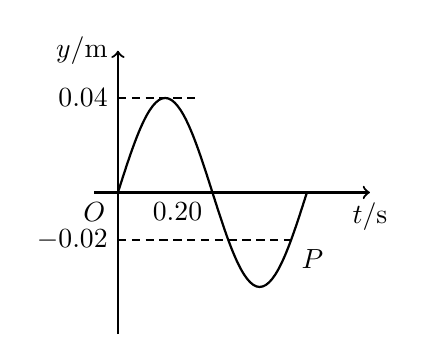
\begin{tikzpicture}
    \draw [->,thick] (-0.3,0) -- (3.2,0) node [anchor=north] {$t/\mathrm{s}$} node [at start,anchor=north] {$O$};
    \draw [->,thick] (0,-1.8) -- (0,1.8) node [anchor=east] {$y/\mathrm{m}$};
    \draw [thick] (0,0) sin (0.6,1.2) cos (1.2,0) node [anchor=north east] {$0.20$} sin (1.8,-1.2) cos (2.4,0);
    \draw [densely dashed,thick] (0,1.2) -- (1,1.2) node [at start,anchor=east] {$0.04$};
    \draw [densely dashed,thick] (0,-.6) -- (2.2,-.6) node [at start,anchor=east] {$-0.02$} node [anchor=north west] {$P$};
\end{tikzpicture}
\vfill
\end{paracol}

\begin{problem}[薄膜干涉]
    一平面単色光在空气中以$i_1=30^\circ$照射到厚度均匀的薄油膜上.油膜覆盖在玻璃板上，所用单色光的波长可以连续变化，观察到$500\mathrm{nm}$ 与$600\mathrm{nm}$这两个波长的光在反射中干涉叠加，亮度显著增强.油的折射率为$1.30$，玻璃的折射率为$1.50$.试求油膜的最小厚度.
\end{problem}
\begin{solution}
\begin{itemize}
    \item 由折射定律$n_1=\sin i_1=n_2\sin i_2$得$\cos i_2=\cos\arcsin\frac{n_1\sin i_1}{n_2}=0.92$.
    \item 设两波长的光在第$k$级叠加增强，光程差满足$2n_2h\cos i_2=k\lambda_1=(k+1)\lambda_2$，则$k$满足的最小正整数为$k=5$.
    \item 将$k=5$代入得油膜的最小厚度$h_{\min}=\frac{k\lambda_1}{2n_2\cos i_2}=1.25\mu\mathrm{m}$.
\end{itemize}
\end{solution}

\begin{paracol}{2}
\begin{problem}[平面简谐波的波函数]
    如图所示为一平面简谐波在$t=2\mathrm{s}$时刻的波形图，$u=0.6\mathrm{m/s}$，求
\begin{enumerate}
    \item 坐标原点$O$质点的振动方程.
    \item 该波的波函数.
    \item $P$点振动方程.
\end{enumerate}
\end{problem}
\switchcolumn\centering
\vfill
\begin{tikzpicture}[decoration={markings,
    mark=between positions 0.05 and 1 step 6mm
    with {\draw [-,gray] (0,-0.1) -- (0,0.1);}}]
    \draw [thick,->,postaction=decorate] (-0.2,0)--(4.2,0) node [anchor=south] {$x/\mathrm{m}$};
    \draw [thick,->] (0,-1.2)--(0,1.5) node [anchor=south] {$y/\mathrm{m}$};
    \node [anchor=north east] at (0,0) {$O$};
    \draw [thick] (0,0) sin (0.6,-1) cos (1.2,0) sin (1.8,1) node [anchor=south] {$t=2\mathrm{s}$} cos (2.4,0) sin (3,-1) cos (3.6,0);
    \draw [very thick,<-] (2.4,1.2)--(3.6,1.2) node [anchor=south,midway] {$u$};
    \node [anchor=north] at (1.2,0) {$0.3$};
    \draw [densely dotted,thick] (0,-1)--(1.2,-1) node [anchor=east,at start] {$0.04$};
    \shade[ball color=H1] (1.2,0) circle (.05) node [anchor=south east] {$P$};
\end{tikzpicture}
\vfill
\end{paracol}
\begin{solution}
\begin{enumerate}
    \item 由图可知振幅$A=0.04\mathrm{m}$，角频率$\omega=\frac{2\pi u}{\lambda}=2\pi$，初相$\varphi=\frac\pi2$. 所以原点的振动方程为\point{2}
    \[y_o=0.04\cos\ab(2\pi(t-2)+\frac\pi2)=0.04\cos\ab(2\pi t+\frac\pi2)\eqno\point{2}\]
    \item $y=0.04\cos\ab[2\pi\ab(t-2+\frac{x}{0.6})+\frac\pi2]=0.04\cos\ab[2\pi\ab(t+\frac{5x}{3})+\frac\pi2]$.\point{3}
    \item 将$x=0.3$代入波函数得$y_p=0.04\cos\ab(2\pi t-\frac\pi2)$.\point{3}
\end{enumerate}
\end{solution}

\begin{problem}[光栅]
    波长为$500\mathrm{nm}$的单色平行光垂直入射到一个透射光栅上，第三级明纹出现在$\sin\theta=0.5$处，第四级缺级. 试求
\begin{enumerate}
    \item 光栅常数$d$是多少？
    \item 光栅上狭缝可能的最小宽度$a$有多大？
    \item 在光屏上观察到最高谱线级次是多少？
    \item 在光屏上可以看到哪些级数的谱线？
\end{enumerate}
\end{problem}
\begin{solution}
\begin{enumerate}
    \item 由光栅方程$d\sin\theta=k\lambda$得$d=\frac{k\lambda}{\sin\theta}=3\mu\mathrm{m}$.\point{3}
    \item 由缺级条件$k'=\frac da$得$a=\frac d4=0.75\mu\mathrm{m}$.\point{2}
    \item 分别令$\sin\theta=\pm 1$得$k=\pm 6$. 由于现实中$\sin\theta$取不到$1$，所以可见最高级次为$5$.\point{3}
    \item $\pm 3$级缺级，所以可见谱线级数有$0,\ \pm1,\ \pm2,\ \pm4,\ \pm5$.\point{2}
\end{enumerate}
\end{solution}

\section*{第3部分（每题15分，共30分）}
\begin{problem}[驻波]
    平面简谐波沿$x$轴正方向传播，频率$f=100\mathrm{Hz}$，振幅$A=0.1\mathrm{m}$，波速$u=100\mathrm{m/s}$.已知在$t=0$时刻，距离坐标原点$x_1=0.5\mathrm{m}$处的质点的位移为$0.1\mathrm{m}$. 当传播到$x_2=2\mathrm{m}$处的固定端时，被全部反射，且反射点是节点. 假设入射波和反射波具有相同的振幅，圆频率和波长. 试求
\begin{enumerate}
    \item 入射波的波函数.
    \item 反射波的波函数.
    \item 合成波的波函数.
    \item 合成波在$0\leq x\leq 2$区间内，波腹和波节点的横坐标.
\end{enumerate}
\end{problem}
\begin{solution}
\begin{enumerate}
    \item $y_1=0.1\cos\ab[200\pi\ab(t-\frac{x-0.5}{100})]=0.1\cos\ab[200\pi\ab(t-\frac{x}{100})+\pi]$.\point{3}
    \item $y_2=0.1\cos\ab[200\pi\ab(t-\frac{2}{100}+\frac{x-2}{100})]=0.1\cos\ab[200\pi\ab(t+\frac{x}{100})]$.\point{5}
    \item $y=y_1+y_2=0.2\cos\ab(200\pi t+\frac\pi2)\cos\ab(2\pi x-\frac\pi2)$.\point{3}
    \item 分别令$\cos\ab(2\pi x-\frac\pi2)=\pm1,\ 0$得此区间内波腹坐标$x=\frac14,\ \frac34,\ \frac54,\ \frac74$，波节坐标$x=0,\ \frac12,\ 1,\ \frac32,\ 2$.\point{4}
\end{enumerate}
\end{solution}

\vskip-2ex
\begin{paracol}{2}
\begin{problem}[简谐振动]
    一个光滑水平面上的弹簧振子，弹簧的劲度系数为$k=900.0\mathrm{N/m}$，弹簧的质量为$m_s=0.3\mathrm{kg}$. 所系物体的质量为$m=0.9\mathrm{kg}$，物块的振幅$A=0.1\mathrm{m}$. 有一质量为$M=8.0\mathrm{kg}$的小物体从高度$h=0.5\mathrm{m}$处自由下落，如图所示. 当振子在最大正位移时，小物体落在物块上，并粘在一起. 假设碰撞在极短时间内完成，也就是碰撞过程中弹簧长度不发生改变. 假定弹簧各截面的位移是线性的. 试求
\begin{enumerate}
    \item 碰撞前，物体经过平衡位置时，物体的速率.
    \item 碰撞前，系统的振动周期.
    \item 碰撞后，物体经过平衡位置时，物体的速率.
    \item 碰撞后，系统的振动周期.
\end{enumerate}
\end{problem}
\switchcolumn\centering
\vfill
\begin{tikzpicture}
    \draw [->] (0,1) -- (0,0) -- (5,0) node [anchor=north] {$x$};
    \draw (2.1,.8) -- (2.1,-.3) node [near end,anchor=north east] {$O$};
    \draw (3,.8) -- (3,-.3) node [near end,anchor=north east] {$A$};
    \draw [decorate,decoration={coil,segment length=3pt}] (0,.3) -- (2.7,.3) node [near start,anchor=south] {$m_2$};
    \filldraw [fill=1号色] (2.7,0) rectangle (3.3,.6);
    \node [anchor=west] at (3.3,.3) {$m$};
    \shade [ball color=H1] (3.3,3) circle (.1) node [anchor=east] {$M$};
    \length{(3.6,.6)}{(3.6,3)}{$h$}{(0,.5)}
\end{tikzpicture}
\vfill
\end{paracol}
\vspace{-.75em}
\begin{solution}
\begin{itemize}
    \item 弹簧的动能$T=\frac12\int_0^l\frac{m_s}{l}\ab(\frac{vx}{l})^2\d x=\frac16m_sv^2=\frac12m_\text{eff}v^2$，由此得弹簧的有效质量$m_\text{eff}=m_s/3$.\point{5}
    \item 周期$T=\frac{2\pi}{\omega}=2\pi\sqrt{\frac{m+m_s/3}{k}}=\frac{\pi}{15}\mathrm{s}$，平衡位置处物体速率$v_0=\frac{2\pi A}{T}=\sqrt{\frac{kA^2}{m+m_s/3}}=3\mathrm{m/s}$.\point{4}
    \item 在最大位移处碰撞不会改变系统的振幅，改变的只有系统的周期 \& 频率.\point{2}
    \item 碰撞后系统周期$T'=2\pi\sqrt{\frac{M+m+m_s/3}{k}}=\frac\pi5$，平衡位置处物体速率$v'=\frac{2\pi A}{T'}=1\mathrm{m/s}$.\point{4}
\end{itemize}
\end{solution}
\kaishu「一项新工作，若可能用四页纸解释清楚，那么我会试一试PRL」\hfill\color{H1}\faIcon{angle-right}~\bfseries 未央物理讲师招新: \mailto{xiamyphys@gmail.com}